\vspace{-0.05in}
\section{Motivation and Background}
\label{background}
\vspace{-0.05in}

\begin{figure}[t]
        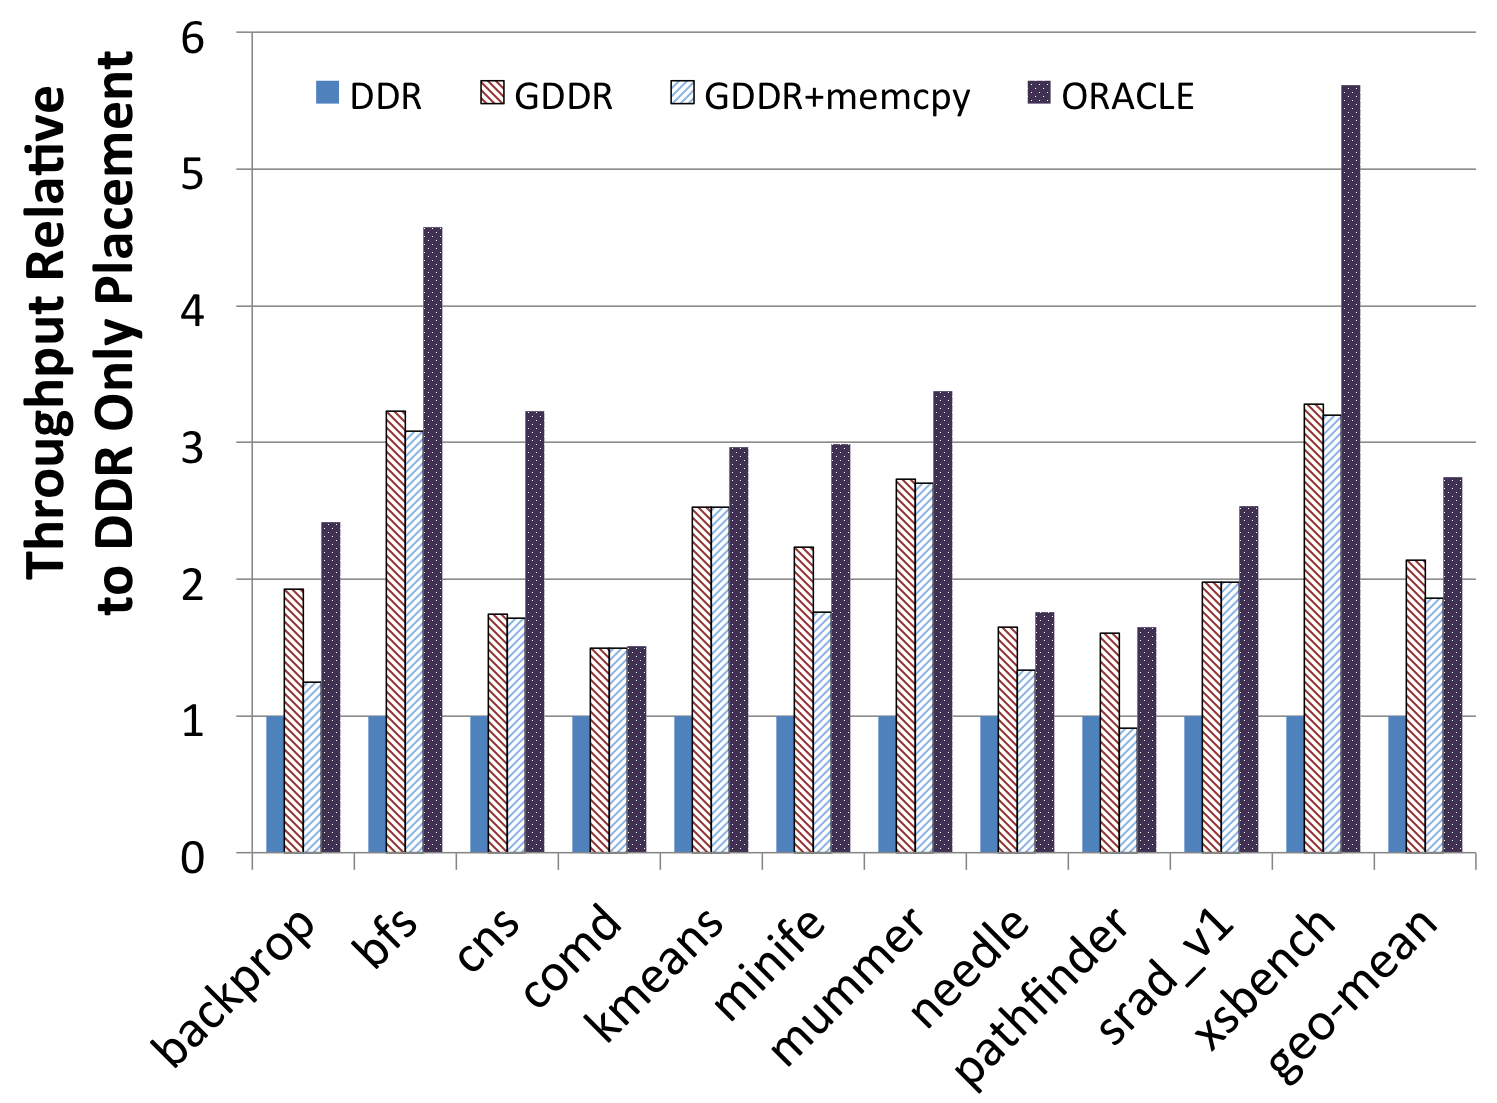
\includegraphics[width=\columnwidth]{hpca2015/figures/motivation.png}
    \caption{GPU performance sensitivity to memory subsystem performance where GDDR provides 
    200GB/s, DDR provides 80GB/s, and {\tt memcpy} bandwidth is 80GB/s.}
    \label{fig:motivation}
\end{figure}

A by-product of the GPU's many-threaded design is that
it is able to maintain a large number of in-flight memory requests and execution throughput
is correlated to memory bandwidth rather than latency, as compared to CPU designs.  As a result,
GPUs have chosen to integrate high bandwidth off-package memory like GDDR rather than accessing
the CPU's DDR directly or integrating DDR locally on the GPU board.  This choice is motivated
by our observation that the performance of some GPU compute workloads would degrade by as much as 
66\% if the traditional GDDR memory on a GPU were replaced with standard DDR memory, as seen in 
Figure~\ref{fig:motivation}.

In current CPU/GPU designs, GPU and CPU memory systems are private and require
explicit copying to the GPU before the application can execute.   Figure~\ref{fig:motivation}
shows the effect of this copy overhead on application performance by comparing GDDR to GDDR+{\tt memcpy}
performance which includes the cost of the programmer manually copying data from the DDR to the GDDR
before launching the GPU kernels.  While this copy overhead varies from application to application,
it can be a non-trivial performance overhead for short-running GPU applications and can even negate the 
effectiveness of using the high bandwidth GDDR on-board the GPU in a limited number of cases.

While it is technically possible for the GPU to access CPU memory directly over PCIe today, the long
latency (microseconds) of the access makes this a rarely used memory operation. 
Programming system
advancements enabling a uniform global address space, like those introduced in
CUDA 6.0~\cite{cuda}, relax the
requirement forcing programmers to allocate and explicitly copy memory to the GPU up-front, but
do nothing to improve the overhead of this data transfer. Further, by copying pages from the CPU to the GPU 
piece-meal on demand, these new runtimes often introduce additional overhead compared to
performing a highly optimized bulk transfer of all the data that the GPU will need during execution.
The next step in the evolution of GPUs, given the unified addressing, is
to optimize the performance of this new programming model. 

\subsection {Cache Coherent GPUs}

The key advancement expected to enable
performance is the introduction of CC-NUMA GPU and CPU systems.  Using cache coherence layered upon NVLink, HT, or QPI, GPUs will
likely be able to access CPU memory in hundreds of nanoseconds at bandwidths up to 128GB/s by bringing
cache lines directly into GPU caches. Figure~\ref{fig:motivation} shows the upper bound (labeled ORACLE) on performance
that could be achieved if both the system DDR memory and GPU GDDR memory were used concurrently, assuming data had 
been optimally placed in both technologies.  In this work, we define oracle placement to be \emph{a priori} page placement
in the GPU memory (thus requiring no migration), of the minimum number of pages, when sorted from hottest to coldest, 
such that the GDDR bandwidth is fully subscribed during application execution.

Because initial CPU/GPU CC-NUMA systems are likely to use a form of IOMMU address translation services 
for walking the OS page tables within the GPU,  it is unlikely that GPUs will be able to directly
allocate and map their own physical memory without a call back to the CPU and operating system.
In this work, we make a baseline assumption that all physically allocated pages are initially allocated
in the CPU memory and only the operating system or GPU runtime system executing on the host can initiate
page migrations to the GPU\@.  In such a system, two clear performance goals become evident.
The first is to design a memory policy that balances CC-NUMA access and page migration to simply achieve the 
performance of the legacy bulk copy interface without the programming limitations.  The second, more ambitious, goal
is to exceed this performance and approach the oracular performance by using these memory zones concurrently, enabling 
a peak memory bandwidth that is the sum of the two zones.

Achieving either of these goals requires
migrating enough data to the GPU to exploit its high memory bandwidth while avoiding migrating pages
that may never be accessed again.  Every page migration increases the total bandwidth requirement of the
application and over-migration potentially reduces application performance if sufficient bandwidth headroom in both the DDR and GDDR is not available.
Thus, the runtime system must be selective about which pages to migrate.  The runtime system also must be cognizant
that performing TLB invalidations (an integral part of page migration) on a GPU does not just halt a single
processor, but thousands of compute pipelines that may be accessing these pages through a large shared TLB structure.
This shared TLB structure makes page migrations between a CPU and GPU potentially much more costly (in terms of the opportunity cost of lost execution throughput) than in CPU-only systems.

In addition to managing the memory bandwidth overhead
of page migration and execution stalls due to TLB shootdowns, the relative bandwidth utilization of both the CPU and GPU memory 
must be taken into account when making page migration decisions.  When trying to balance memory bandwidth between two distinct memory
zones, it is possible to over- or under-subscribe either memory zone. Migrating pages too slowly to the GPU
memory will leave its local memory sitting idle, wasting precious bandwidth.  Conversely, migrating pages
to the GPU too aggressively may result in under-utilization of the CPU memory while paying the maximum cost in terms
of migration overheads. A comprehensive CPU-GPU memory management solution will attempt to balance all of 
these effects to maximize memory system and GPU throughput in future mobile, graphics, HPC, and datacenter
installations.

\subsection{Related Work}
\label{related_work}
\vspace{-0.05in}

Using mixed DRAM technologies or DRAM in conjunction with non-volatile memories
to improve power consumption on CPUs has been explored by several groups
~\cite{Kultursay2013,Phadke11mlpaware2011,Mogul2009,Bheda2011,Ramos2011}.
The majority of this work attempts to overcome the performance reductions introduced
by non-DDR technologies to improve capacity, power consumption, or both.
In CC-NUMA systems, there has been a long tradition of examining where to place
memory pages and processes for optimal performance, typically focusing on reducing
memory latency~\cite{Wilson2001,Bolosky1989,Brecht1993,LaRowe1992,Verghese1996,Iyer1998}.
Whereas CPUs are highly sensitive to memory latency, GPUs can cover a much larger latency
through the use of multi-threading.  More recent work on page placement and 
migration~\cite{AUTONUMA,Dashti2013,Tam2007,Zhuravlev2010,Knauerhase2008,Blagodurov2011,awasthinellans10}
has considered data sharing characteristics, interconnect utilization, and memory controller
queuing delays in the context of CPU page placement. However, the primary improvements in many of these works,
reducing average memory latency, will not directly apply in a GPU optimized memory system.

Several recent papers have explored hybrid DRAM-NVM GPU attached memory subsystems~\cite{zhao2013,Wang2013}.
Both of these works consider a traditional GPU model where the availability of low latency, high bandwidth access to CPU-attached 
memory is not considered, nor are the overheads of moving data from the host CPU onto the GPU considered.
Several papers propose using a limited capacity, high bandwidth memory as a
cache for a larger slower memory~\cite{jiang2011,Meza2012}, but such designs incur a high engineering
overhead and would require close collaboration between GPU and CPU vendors that often do not
have identically aligned visions of future computing systems.

When designing page migration policies, the impact of TLB shootdown overheads and page table updates is a constant
issue.  Though most details about GPU TLBs are not public,
several recent papers have provided proposals about how to efficiently implement general purpose TLBs
that are, or could be, optimized for a GPU's needs~\cite{Pichai2014,Villavieja2011,Power2014}. Others
have recently looked at improving TLB reach by exploiting locality within the virtual to physical
memory remapping, or avoiding this layer completely~\cite{swansonstoller98,Pham2014,Basu2013}.  
Finally, Gerofi et al.~\cite{Gerofi2014} recently examined TLB performance of the Xeon Phi
for applications with large footprints, while McCurdy et al.~\cite{McCurdy2008} investigated the
effect of superpages and TLB coverage for HPC applications in the context of CPUs.
